\documentclass[a4paper,11pt]{article}

\usepackage[utf8]{inputenc}
\usepackage[italian]{babel}
\usepackage{default}
\usepackage{amssymb}
\usepackage{amsmath}
\usepackage{amsthm}
\usepackage{hyperref}
\usepackage{textcomp}
\usepackage{tikz}
\usepackage{graphicx}
\usepackage{caption}
\usepackage{subcaption}
\usepackage[export]{adjustbox}


\newcommand{\Near}{\mathcal{N}}
\newcommand{\Surr}{\mathcal{S}}
\newcommand{\A}{\mathcal{A}}
\newcommand{\E}{\mathcal{E}}
\renewcommand{\(}{\left(}
\renewcommand{\)}{\right)}
\newcommand{\<}{\textlangle}
\renewcommand{\>}{\textrangle}


\title{Model Checker per la logica STL}
\author{Gianluca Grilletti}

\begin{document}

\maketitle

\pagebreak

Nel seguente documento vengono presentati brevemente la sintassi della logica STL (\emph{space-temporal logic}) e i comandi principali del modelchecker che implementa tale logcia. Viene in seguito presentato un esempio d'uso del model checker commentato.

In seguito verranno utilizzate le notazioni introdotte in \cite{ciancia} sugli spazi topologici quasi-discreti.


\section{La logica STL}

La sintassi della logica STL è data dalla seguente grammatica, dove $p$ varia tra un insieme $P$ di proposizioni atomiche

\begin{gather}
 \Phi ::= p \,|\, \perp \,|\, \neg \Phi \,|\, \Phi \wedge \Phi \,|\, \Near \Phi \,|\, [\Phi] \Surr [\Phi] \,|\, E \Psi \,|\, A \Psi \\
 \Psi ::= X \Phi \,|\, F \Phi \,|\, [\Phi ] U [\Phi ]
\end{gather}

Un modello per tale logica è una struttura $ M = ( ( X , C ) , ( S , R ) , V_{s\in S} ) $ dove
\begin{itemize}
 \item $(X,C)$ è uno spazio topologico quasi-discreto
 \item $(S,R)$ è un \emph{Kripke frame}
 \item $V_s$ è una funzione da $P$ (l'insieme delle proposizioni atomiche) a $\mathcal{P} (X)$
\end{itemize}

Nel seguito ci riferiremo ad $X$ come allo spazio del modello, ad $S$ come al tempo, a $s\in S$ come ad un istante ed a $V$ come all'ambiente del modello.

Quello che rappresenta un modello è uno spazio su cui possono essere valutate delle proprietà. Tali proprietà possono però variare nel tempo ed abbiamo quindi bisongo di avere una struttura temporale che descriva tale cambiamento.

Nel seguito con $\mathcal{P}_s$ indicheremo le sequenze infinite di istanti che partono da $s$. Dato $\sigma \in \mathcal{P}_s$, con $\sigma(n)$ indichiamo l'$n$-esimo istante della sequenza. La valutazione semantica in un certo punto dello spazio $x$, per un certo istante $s$ è data dalle seguenti clausole induttive
\begin{itemize}
 \item $M,x,s \not \vDash \perp$
 \item $M,x,s \vDash p$ se e solo se $x\in V_s(p)$
 \item $M,x,s \vDash \neg \phi$ se e solo se $M,x,s \not\vDash \phi$
 \item $M,x,s \vDash \phi \wedge \psi$ se e solo se $M,x,s \vDash \phi$ e $M,x,s \vDash \psi$
 \item $M,x,s \vDash \Near \phi$ se e solo se \[ x\in C \( \{ y\in X \mid M,y,s\vDash \phi \} \) \]
 \item $M,x,s \vDash [\phi] S [\psi]$ se e solo se \[ \exists A \subseteq X . x\in A \wedge \forall y \in A . M,y,s\vDash \phi \wedge \forall z \in \mathcal{B}^+(A).M,z,s\vDash \psi \]
 \item $M,x,s \vDash A\phi $ se e solo se $\forall \sigma \in \mathcal{P}_s . M,x,\sigma \vDash $
 \item $M,x,s \vDash E\phi $ se e solo se $\exists \sigma \in \mathcal{P}_s . M,x,\sigma \vDash $
 \item $M,x,\sigma \vDash X\phi$ se e solo se $M,x,\sigma(1) \vDash \phi$
 \item $M,x,\sigma \vDash [\phi] U [\psi]$ se e solo se $\exists n . M,x,\sigma(n) \vDash \psi$ e $\forall n' < n . M,x,\sigma(n') \vDash \phi$
 \item $M,x,\sigma \vDash F \phi$ se e solo se $\exists n . M,x,\sigma(n) \vDash \psi$
\end{itemize}

Si può mostrare in particolare che con questa semantica le formule $\perp$, $p$, $\Phi \wedge \Phi$, $\neg \Phi$, $\Near \Phi$, $[\Phi] \Surr [\Phi]$, $EX \Phi$, $AF \Phi$ ed $E[\Phi]U[\Phi]$ sono una base della logica introdotta.

Altri operatori che possono essere definiti sono
\begin{itemize}
 \item $AG \phi ::= \neg ( E [T ] U [\neg \phi ] )$
 \item $EG \phi ::= \neg AF (\neg \phi) $
\end{itemize}


\section{Il model checker}

Definiamo un modello finito se $X$ e $S$ sono finiti. Dato un modello $M$ finito il model checker introdotto permette di testare formule della logica STL su $M$. In particolare la valutazione di una formula $\phi$ restituisce l'insieme delle coppie $(x,s)$ tali che $M,x,s\vDash \phi$.

Nell'implementazione attuale si assume che lo spazio sia una griglia $m \times n$ ottenuta caricando un'immagine od una serie di immagini. Il model checker mostra in maniera interattiva l'immagine relativa ad un certo istante di tempo deciso dall'utente. Valutando una formula i punti che la verificano vengono colorati.

Durante l'esecuzione possono essere fissati un punto dello spazio $s_0$, un istante di tempo $t_0$ ed una formula $f_0$, in modo da poter controllare la validita della formula sui singoli punti oltre che visivamente sull'immagine.

Diamo ora i comandi del model checker:
\begin{description}
  \item[show store;] Mostra le formule attualmente salvate in memoria.
  \item[show status;] Restituisce posizione, tempo e formula zero. Inoltre restituisce la valutazione della formula zero nella posizione e nel tempo zero.
  \item[show future;] Mostra i possibili tempi futuri e la valutazione della formula zero nella posizione zero.
  \item[show space;] Mostra la posizione zero. Sulla mappa, colora un pixel corrispondente alla posizione zero.
  \item[show time;] Mostra il tempo zero.
  \item[show formula;] Mostra la formula zero.
  \item[set space \<int\> \<int\>;] Imposta la posizione zero.
  \item[set time \<int\>;] Imposta il tempo zero e carica l'immagine corrispondente.
  \item[let \<ide\> = \<fsyntax\>;] Definisce una nuova formula e la salva nello store.
  \item[sem \<color\> \<ide\>;]
  \item[sem \<color\> \<ide\> \<fsyntax\> ... \<fsyntax\>;]
  \item[sem \<color\> \<fsyntax\>;] Colora i punti in cui la formula richiamata risulta vera (per richiamare formule con parametri serve definirle precedentemente col comando let).
  \item[save store;] Salva lo store attuale nel file formula.fr (cancella eventuali dati precedentemente salvati).
  \item[load store;] Carica lo store salvato in formula.fr
  \item[save image \<filename\>;] Salva lo stato attuale del sistema. [save image prova;] salva una bitmap per ogni punto del tempo (ad esempio, al punto 2 corrisponde il file prova2.bmp)
  \item[reset;] Riporta il sistema allo stato di avvio.
  \item[refresh;] Ricarica l'immagine.
  \item[exit;] Ferma il programma.
\end{description}

\pagebreak




\section{Un esempio}


Forniamo ora un esempio di utilizzo del model checker. Nel nostro esempio il Kripke frame è il seguente

\begin{tikzpicture}

  \node at (0,0) {};

  \node (0) at (0,-2) [circle,draw=black] {0};
  \foreach \i in {1,...,5}
  {
    \pgfmathtruncatemacro{\p}{\i-1}
    \node (\i) at (\i,-2) [circle,draw=black] {\i};
    \draw [->] (\p) -- (\i);
  }
  
  \node (6) at (6,-1) [circle,draw=black] {6};
  \draw [->] (5) -- (6);
  \foreach \i in {7,...,10}
  {
    \pgfmathtruncatemacro{\p}{\i-1}
    \node (\i) at (\i,-1) [circle,draw=black] {\i};
    \draw [->] (\p) -- (\i);
  }
  
  \node (11) at (6,-3) [circle,draw=black] {11};
  \draw [->] (5) -- (11);
  \foreach \i in {12,...,15}
  {
    \pgfmathtruncatemacro{\p}{\i-1}
    \pgfmathtruncatemacro{\j}{\i-5}
    \node (\i) at (\j,-3) [circle,draw=black] {\i};
    \draw [->] (\p) -> (\i);
  }
  
  \foreach \i in {0,...,15}
  {
    \draw (\i) edge [loop below,->] node {} (\i);
  }
  
\end{tikzpicture}

cioè ci sono due possibili evoluzioni per il futuro all'istante 5.


La sequenza di immagini caricate è
\begin{figure}[htp]
\centering

\includegraphics[width=.15\textwidth,frame]{images/start1.png} 1

\includegraphics[width=.15\textwidth,frame]{images/start2.png} 2

\includegraphics[width=.15\textwidth,frame]{images/start3.png} 3

\includegraphics[width=.15\textwidth,frame]{images/start4.png} 4

\includegraphics[width=.15\textwidth,frame]{images/start5.png} 5
\\

\includegraphics[width=.15\textwidth,frame]{images/start6.png} 6

\includegraphics[width=.15\textwidth,frame]{images/start7.png} 7

\includegraphics[width=.15\textwidth,frame]{images/start8.png} 8

\includegraphics[width=.15\textwidth,frame]{images/start9.png} 9

\includegraphics[width=.15\textwidth,frame]{images/start10.png} 10
\\

\includegraphics[width=.15\textwidth,frame]{images/start11.png} 11

\includegraphics[width=.15\textwidth,frame]{images/start12.png} 12

\includegraphics[width=.15\textwidth,frame]{images/start13.png} 13

\includegraphics[width=.15\textwidth,frame]{images/start14.png} 14

\includegraphics[width=.15\textwidth,frame]{images/start15.png} 15
\label{figure:1}
\caption{Figure 1}
\end{figure}

Il centro del cerchio nelle figure si sta muovendo a velocità costante verso destra. Il suo raggio cresce a velocità costante $v$ dalla figura 1 alla figura 5. Nel primo futuro (figure da 6 a 10) il raggio continua a crescere, mentre nel secondo futuro (figure da 11 a 15) il raggio diminuisce a velocità costante $v$.

Le proposizioni atomiche sono $g$ ed $r$ che valutate restituiscono rispettivamente i punti verdi ed i putni rossi nelle figure.

La valutazione della formula $[g]S[r]$ è restituita dal comando

\verb| sem blue S[<g>,<r>]|

\begin{figure}[htp]
\centering

\includegraphics[width=.15\textwidth,frame]{images/surrgreenred1.png} 1

\includegraphics[width=.15\textwidth,frame]{images/surrgreenred2.png} 2

\includegraphics[width=.15\textwidth,frame]{images/surrgreenred3.png} 3

\includegraphics[width=.15\textwidth,frame]{images/surrgreenred4.png} 4

\includegraphics[width=.15\textwidth,frame]{images/surrgreenred5.png} 5
\\

\includegraphics[width=.15\textwidth,frame]{images/surrgreenred6.png} 6

\includegraphics[width=.15\textwidth,frame]{images/surrgreenred7.png} 7

\includegraphics[width=.15\textwidth,frame]{images/surrgreenred8.png} 8

\includegraphics[width=.15\textwidth,frame]{images/surrgreenred9.png} 9

\includegraphics[width=.15\textwidth,frame]{images/surrgreenred10.png} 10
\\

\includegraphics[width=.15\textwidth,frame]{images/surrgreenred11.png} 11

\includegraphics[width=.15\textwidth,frame]{images/surrgreenred12.png} 12

\includegraphics[width=.15\textwidth,frame]{images/surrgreenred13.png} 13

\includegraphics[width=.15\textwidth,frame]{images/surrgreenred14.png} 14

\includegraphics[width=.15\textwidth,frame]{images/surrgreenred15.png} 15
\label{figure:2}
\caption{Figure 2}
\end{figure}

e colora la regione verde avente bordo rosso (\ref{figure:2}).

Il comando

\verb| sem blue S[!(<g> or <r>),<r>] |

\begin{figure}[htp]
\centering

\includegraphics[width=.15\textwidth,frame]{images/whitetoblu1.png} 1

\includegraphics[width=.15\textwidth,frame]{images/whitetoblu2.png} 2

\includegraphics[width=.15\textwidth,frame]{images/whitetoblu3.png} 3

\includegraphics[width=.15\textwidth,frame]{images/whitetoblu4.png} 4

\includegraphics[width=.15\textwidth,frame]{images/whitetoblu5.png} 5
\\

\includegraphics[width=.15\textwidth,frame]{images/whitetoblu6.png} 6

\includegraphics[width=.15\textwidth,frame]{images/whitetoblu7.png} 7

\includegraphics[width=.15\textwidth,frame]{images/whitetoblu8.png} 8

\includegraphics[width=.15\textwidth,frame]{images/whitetoblu9.png} 9

\includegraphics[width=.15\textwidth,frame]{images/whitetoblu10.png} 10
\\

\includegraphics[width=.15\textwidth,frame]{images/whitetoblu11.png} 11

\includegraphics[width=.15\textwidth,frame]{images/whitetoblu12.png} 12

\includegraphics[width=.15\textwidth,frame]{images/whitetoblu13.png} 13

\includegraphics[width=.15\textwidth,frame]{images/whitetoblu14.png} 14

\includegraphics[width=.15\textwidth,frame]{images/whitetoblu15.png} 15
\label{figure:3}
\caption{Figure 3}
\end{figure}

colora invece la regione bianca (non verde e non rossa) avente bordo rosso (\ref{figure:3}).

Il comando

\verb| sem blue AG <g> |

restituisce i punti che per \emph{qualsiasi futuro} saranno verdi in ogni istante.

\begin{figure}[htp]
\centering
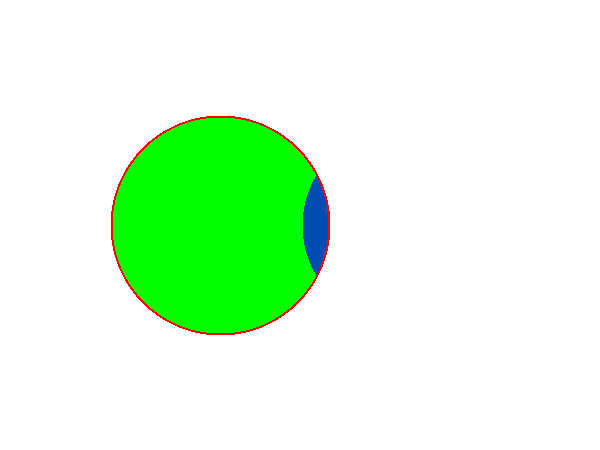
\includegraphics[width=.15\textwidth,frame]{images/aggreen1.png} 1
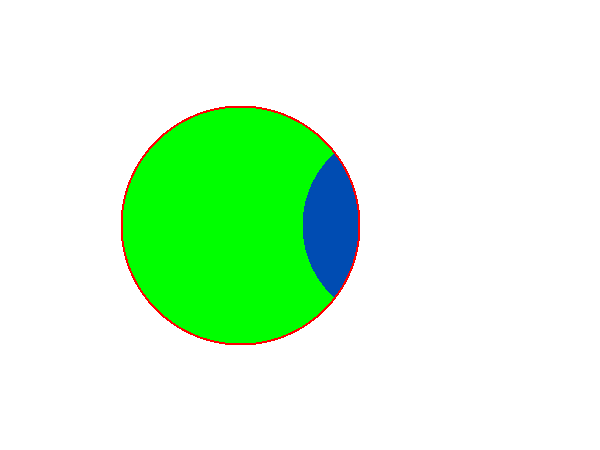
\includegraphics[width=.15\textwidth,frame]{images/aggreen2.png} 2
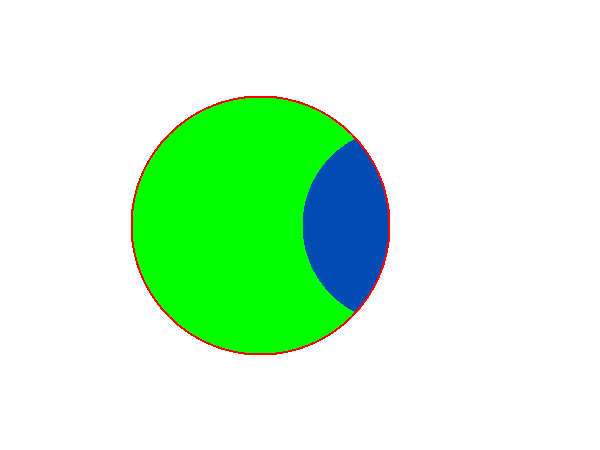
\includegraphics[width=.15\textwidth,frame]{images/aggreen3.png} 3
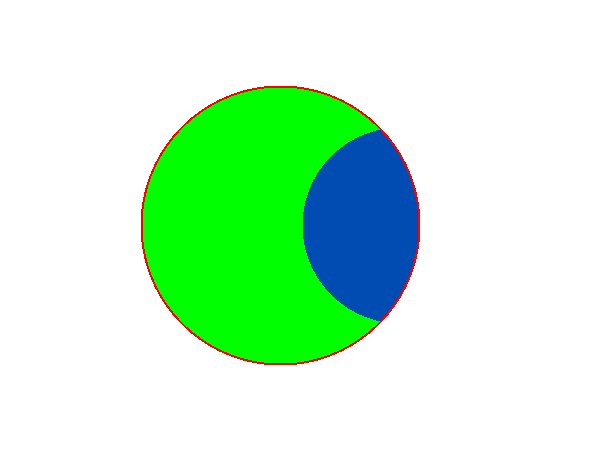
\includegraphics[width=.15\textwidth,frame]{images/aggreen4.png} 4
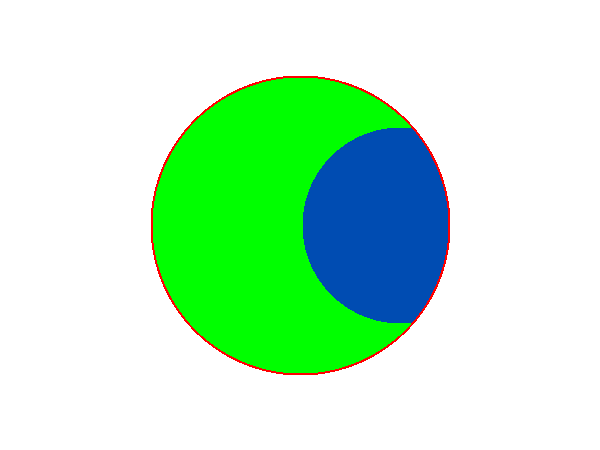
\includegraphics[width=.15\textwidth,frame]{images/aggreen5.png} 5
\\
\includegraphics[width=.15\textwidth,frame]{images/aggreen6.png} 6
\includegraphics[width=.15\textwidth,frame]{images/aggreen7.png} 7
\includegraphics[width=.15\textwidth,frame]{images/aggreen8.png} 8
\includegraphics[width=.15\textwidth,frame]{images/aggreen9.png} 9
\includegraphics[width=.15\textwidth,frame]{images/aggreen10.png} 10
\\
\includegraphics[width=.15\textwidth,frame]{images/aggreen11.png} 11
\includegraphics[width=.15\textwidth,frame]{images/aggreen12.png} 12
\includegraphics[width=.15\textwidth,frame]{images/aggreen13.png} 13
\includegraphics[width=.15\textwidth,frame]{images/aggreen14.png} 14
\includegraphics[width=.15\textwidth,frame]{images/aggreen15.png} 15
\label{figure:4}
\caption{Figure 4}
\end{figure}

Notiamo che la valutazione sulle figure dalla 1 alla 5 risulta essere l'intersezione di due cerchi (quello della figura considerata e quello in figura 15). Nelle figure da 11 a 15 la situazione è la stessa in quanto l'istante 15 è ancora un possibile istante futuro. Invece nelle figure da 6 a 10 l'istante 15 non è più raggiungibile e quindi l'area che rimarrà definitivamente verde si amplia.










\pagebreak

\begin{thebibliography}{9}

	\bibitem{ciancia}
  Vincenzo Ciancia, Diego Latella, Michele Loreti, Mieke Massink
  \emph{Specifying and Verifying Properties of Space}.
  16 Maggio 2014
  
\end{thebibliography}




\end{document}
